% -*- mode: LaTeX; TeX-PDF-mode: t; -*-
\providecommand{\econtexRoot}{}
\renewcommand{\econtexRoot}{..}
\providecommand{\econtexPaths}{}\renewcommand{\econtexPaths}{\econtexRoot/Resources/econtexPaths}
% The \commands below are required to allow sharing of the same base code via Github between TeXLive on a local machine and Overleaf (which is a proxy for "a standard distribution of LaTeX").  This is an ugly solution to the requirement that custom LaTeX packages be accessible, and that Overleaf prohibits symbolic links

\providecommand{\econtex}{\econtexRoot/Resources/texmf-local/tex/latex/econtex}
\providecommand{\pdfsuppressruntime}{\econtexRoot/Resources/texmf-local/tex/latex/pdfsuppressruntime}
\providecommand{\econark}{\econtexRoot/Resources/texmf-local/tex/latex/econark}
\providecommand{\econtexSetup}{\econtexRoot/Resources/texmf-local/tex/latex/econtexSetup}
\providecommand{\econtexShortcuts}{\econtexRoot/Resources/texmf-local/tex/latex/econtexShortcuts}
\providecommand{\econtexBibMake}{\econtexRoot/Resources/texmf-local/tex/latex/econtexBibMake}
\providecommand{\econtexBibStyle}{\econtexRoot/Resources/texmf-local/bibtex/bst/econtex}
\providecommand{\econtexBib}{economics}
\providecommand{\economics}{\econtexRoot/Resources/texmf-local/bibtex/bib/economics}
\providecommand{\notes}{\econtexRoot/Resources/texmf-local/tex/latex/handout}
\providecommand{\handoutSetup}{\econtexRoot/Resources/texmf-local/tex/latex/handoutSetup}
\providecommand{\handoutShortcuts}{\econtexRoot/Resources/texmf-local/tex/latex/handoutShortcuts}
\providecommand{\handoutBibMake}{\econtexRoot/Resources/texmf-local/tex/latex/handoutBibMake}
\providecommand{\handoutBibStyle}{\econtexRoot/Resources/texmf-local/bibtex/bst/handout}

\providecommand{\FigDir}{\econtexRoot/Figures}
\providecommand{\CodeDir}{\econtexRoot/Code}
\providecommand{\DataDir}{\econtexRoot/Data}
\providecommand{\SlideDir}{\econtexRoot/Slides}
\providecommand{\TableDir}{\econtexRoot/Tables}
\providecommand{\ApndxDir}{\econtexRoot/Appendices}

\providecommand{\ResourcesDir}{\econtexRoot/Resources}
\providecommand{\rootFromOut}{..} % APFach back to root directory from output-directory
\providecommand{\LaTeXGenerated}{\econtexRoot/LaTeX} % Put generated files in subdirectory
\providecommand{\econtexPaths}{\econtexRoot/Resources/econtexPaths}
\providecommand{\LaTeXInputs}{\econtexRoot/Resources/LaTeXInputs}
\providecommand{\LtxDir}{LaTeX/}
\providecommand{\EqDir}{Equations} % Put generated files in subdirectory

% \owner determines where links to online content go
% llorracc is Chris Carroll's personal version
% econ-ark is the Econ-ARK/REMARK version
%\providecommand{\owner}{llorracc}
\providecommand{\owner}{econ-ark}

\documentclass[pdflatex]{beamer}
\usepackage{ifthen}
\newboolean{Web}\setboolean{Web}{false}
\usepackage{econark}
\providecommand{\texname}{BufferStockTheory-Slides}% 

% Can't read in BufferStockTheory.sty because some packages conflict with Beamer
% So need to redefine everything here

\usepackage{econark}
\usepackage{\econtexShortcuts}
\usepackage{\LaTeXInputs/\texname}

\setboolean{showPageHead}{false}

\usepackage{natbib,amsmath,amssymb,rotating,subfigure}
\usepackage{verbatim,moreverb,graphicx}
\usepackage{wasysym}
\usepackage{dcolumn}
\usepackage{cancel}
%\renewcommand{\LtxDir\EqDir}{\econtexRoot/Equations}
\providecommand{\FigsRaw}{\econtexRoot/Code/Python/Figures}
\providecommand{\CodeDir}{\econtexRoot/Code}
\providecommand{\CalibrationDir}{\econtexRoot/Calibration}
\providecommand{\TableDir}{\econtexRoot/Tables}
\providecommand{\ApndxDir}{\econtexRoot/Appendices}
\providecommand{\Ex}{\mathbb{E}}


%\usepackage{natbib}\newcommand*{\newblock}{}

\mode<presentation>
{
  \usetheme{Warsaw}
  % or ...
  \setbeamercovered{transparent}
}

%\beamerdefaultoverlayspecification{<+->}

%\setbeamertemplate{navigation symbols}{}  % Take away navigation symbols

\usetheme{Warsaw}

\setbeamersize{text margin left=3mm}
\setbeamersize{text margin right=3mm}


%_____________ Opening slide _______________________

\title[Buffer Stock Theory]{Theoretical Foundations of Buffer Stock Saving}
\author[Carroll]{Chris Carroll}
\institute[JHU]{Johns Hopkins University}
\date[\today]{September 12, 2019  \\ \medskip \medskip \medskip \href{https://econ-ark.org/}{\small Powered By} \\ 
\includegraphics[width=0.5in]{\econtexRoot/Resources/econ-ark-logo-small.png}}

\begin{document}\bibliographystyle{\econtexBibStyle}

\begin{frame}[plain]
  \titlepage
\end{frame}


%_____________ 1st section  ____________
\section{Introduction}
\subsection{Motivation}

\begin{frame}
\frametitle{Drawbacks of Numerical Solutions}


\pause A Black Box \pause
\begin{itemize}
\item Can Construct Solution to Model Without Really Understanding It
\item Hard Even To Be Sure Your Numerical Solution Is {\it Right}
\item Little Intuition for How Results Might Change With
\begin{itemize}
\item Calibration
\item Structure
\end{itemize}
\item {\it Very} Hard To Teach!
\end{itemize}

\medskip\medskip
\pause I Am A {\it Big} Fan Of Numerical Methods
\begin{itemize}
\item Have Done A Good Deal Of Work With Them Myself
\item But As A Result, Have Felt All These Drawbacks Keenly
\end{itemize}



\end{frame}

\begin{frame}
\frametitle{The Gap This Paper Fills}

\pause Foundations For Microeconomic Household's Problem With
\begin{itemize}
\item Uncertain Labor Income
\item No Liquidity Constraints
\item CRRA Utility
\item (Problem with Liquidity Constraints Is A Limiting Case)
\end{itemize}

\end{frame}
\begin{frame}{Key Result}
\pause
Restrictions On Parameter Values Such That \pause
\begin{itemize}
\item Problem Defines A Contraction Mapping
\begin{itemize}
\item $\Rightarrow~~\exists $ A Unique Consumption Function $\cFunc(\mNrm)$
\end{itemize}
\item There Is A `Target' Ratio Of Assets to Permanent Income
\begin{itemize}
\item Requires A Key `Impatience' Condition To Hold
\item Good News
\begin{itemize} \item Condition Is Weaker (Easier To Satisfy) Than Previous Papers Imposed \end{itemize}
\end{itemize}
\end{itemize}

\end{frame}

\section{The Problem}

\begin{frame}

Limit as horizon $T$ goes to infinity of 
  \begin{align*}
    \vLevBF_{T-n} & = \max~ \Ex_{t}\left[\sum_{i=0}^{n} \DiscFac^{i} \uFunc(\cLevBF_{t+i})\right]
  \end{align*}


    \begin{equation}\label{eq:DBCparts}
      a  = 1
    \end{equation}


  \begin{equation}
    \TranShkAll _{t+n}=
    \begin{cases}
      0\phantom{_{t+1}/\pNotZero} & \text{with probability $\pZero>0$} \\
      \TranShkEmp_{t+n}/\pNotZero      & \text{with probability $\pNotZero  $} % \equiv (1-\pZero)
    \end{cases} \label{eq:TranShkDef}
  \end{equation}


\begin{itemize}
\item $\util(\bullet)=\bullet^{1-\CRRA}/(1-\CRRA)$; $\Ex_{t}[\PermShk_{t+n}]=\Ex_{t}[\TranShk_{t+n}]=1~\forall~n>0$; $\beta < 1, \CRRA > 1$
\end{itemize}

\end{frame}

\begin{frame}
\frametitle{Surely This Problem Has Been Solved?}

\pause No.
\begin{itemize}
\item Can't Use Stokey et.\ al.\ theorems because CRRA utility
\item Lit thru \cite{mnUnique} Can't Handle Permanent Shocks
\item Must Use Boyd's `Weighted' Contraction Mapping Theorem 
\item Surprisingly Subtle
\end{itemize}

\pause Fortunately, the Conclusions Are Simple!

\end{frame}

\subsection{The Perfect Foresight Problem}

\begin{frame}
\frametitle{Benchmark: Perfect Foresight Model}

Definitions: \smallskip

\begin{tabular}{llcl}
   Absolute Patience Factor & $\APFac$ & = & $(\Rfree \Discount)^{1/\CRRA}$
\\ Return Patience Factor & $\RPFac$ & = & $\APFac/\Rfree$
\\ Perfect Foresight Growth Patience Factor & $\GPFacRaw$ & = & $\APFac/\PermGroFac$
\end{tabular}

\medskip

\begin{tabular}{l|lcl|l} \hline
   Name                                 & \multicolumn{3}{c|}{Condition}    & Implication 
\\ \hline ($\AIC$) Absolute Impatience Condition  & $\APFac$  & $<$ & 1 & $\cLvl$ $\downarrow$ over time
\\ ($\RIC$) Return Impatience Condition    & $\RPFac$ & $<$ & 1 & $\cLvl/\aLvl$ $\downarrow$ over time
\\ ($\GICRaw$) Growth Impatience Condition & $\GPFacRaw$ & $<$ & 1 & $\cLvl/\PermLvl$ $\downarrow$ over time
\end{tabular}

\medskip

\end{frame}

\begin{frame}
\frametitle{When Does A Useful Limiting Solution Exist?}

Finite Human Wealth ($\FHWC$) condition:
\begin{eqnarray}
\PermGroFac & < & \Rfree
\end{eqnarray}

\pause\medskip
Return Impatience Condition:
\begin{eqnarray}
\RPFac & < & \Rfree
\end{eqnarray}

\end{frame}

\begin{frame}
\frametitle{What If There Are Liquidity Constraints?}

\pause 

\begin{itemize}
\item \FHWC~is {\it not} necessary for solution to exist
\item Other Key Condition For Useful Solution is

`Perfect Foresight Finite Value of Autarky Condition (\PFFVAC)':
\begin{eqnarray}
\beta \PermGroFac^{1-\CRRA} & < & 1  
\end{eqnarray}

\item Without \RIC, Constraints Are Irrelevant
\begin{itemize}
\item Because Wealth Always Wants To Rise, So Constraint Never Binds
\end{itemize}
\end{itemize}

\end{frame}

\begin{frame}
\frametitle{Liquidity Constraints and Uncertainty}

\begin{itemize}
\item Introduce permanent shocks to income
\item Finite Value of Autarky Condition Becomes
\input \EqDir/FVAC
\end{itemize}

\end{frame}



\subsection{The Real Problem}
\begin{frame}
\frametitle{Contraction Mapping Requirements}

Finite Value of Autarky Condition: Same As In Liq Constr Problem!
\input \LtxDir\EqDir/FVAC

`Weak Return Impatience Condition' ($\WRIC$)

\begin{eqnarray}
 0 \leq & \pZero^{1/\CRRA} \RPFac & < 1 \label{eq:WRIC}
\end{eqnarray}

\end{frame}

\begin{frame}
\frametitle{Requirement For Existence Of A Target}

Definitions: `Uncertainty-Adjusted' Growth:
\input \LtxDir\EqDir/PermGroFacAdj

Adjusted Growth Patience Factor:
\input \LtxDir\EqDir/GPFacNrm

Growth Impatience Condition:
\input \LtxDir\EqDir/GICNrm~



Why?  Because it can be shown that
\begin{eqnarray}
 \lim_{\mNrm_{t} \rightarrow \infty} \Ex_{t}\left[\frac{\mNrm_{t+1}}{\mNrm_{t}}\right] & = & \GPFacNrm  \label{eq:mGrowth}
\end{eqnarray}

\end{frame}

\section{Features Of the Solution}
\subsection{Five Propositions}
\begin{frame}
\frametitle{Five Propositions}

\begin{enumerate}
\item $\lim_{\mNrm_{t} \rightarrow \infty} \Ex_{t}[\cLvl_{t+1}/\cLvl_{t}] = \APFac$
\item $\lim_{\mNrm_{t} \rightarrow 0} \Ex_{t}[\cLvl_{t+1}/\cLvl_{t}] = \infty$
\item $\exists$ a unique target value of $\mNrm$, called $\check{\mNrm}$
\item $\Ex_{t}[\cLvl_{t+1}/\cLvl_{t} | \mNrm_{t} = \check{m}] = \PermGroFac - \epsilon$
\item $\left(\frac{d \Ex_{t}[\cLvl_{t+1}/\cLvl_{t}]}{d \mNrm_{t}}\right) < 0$
\end{enumerate}

\end{frame}

\subsection{The Target Saving Figure}
\begin{frame}
\frametitle{The Target Saving Figure}
\centerline{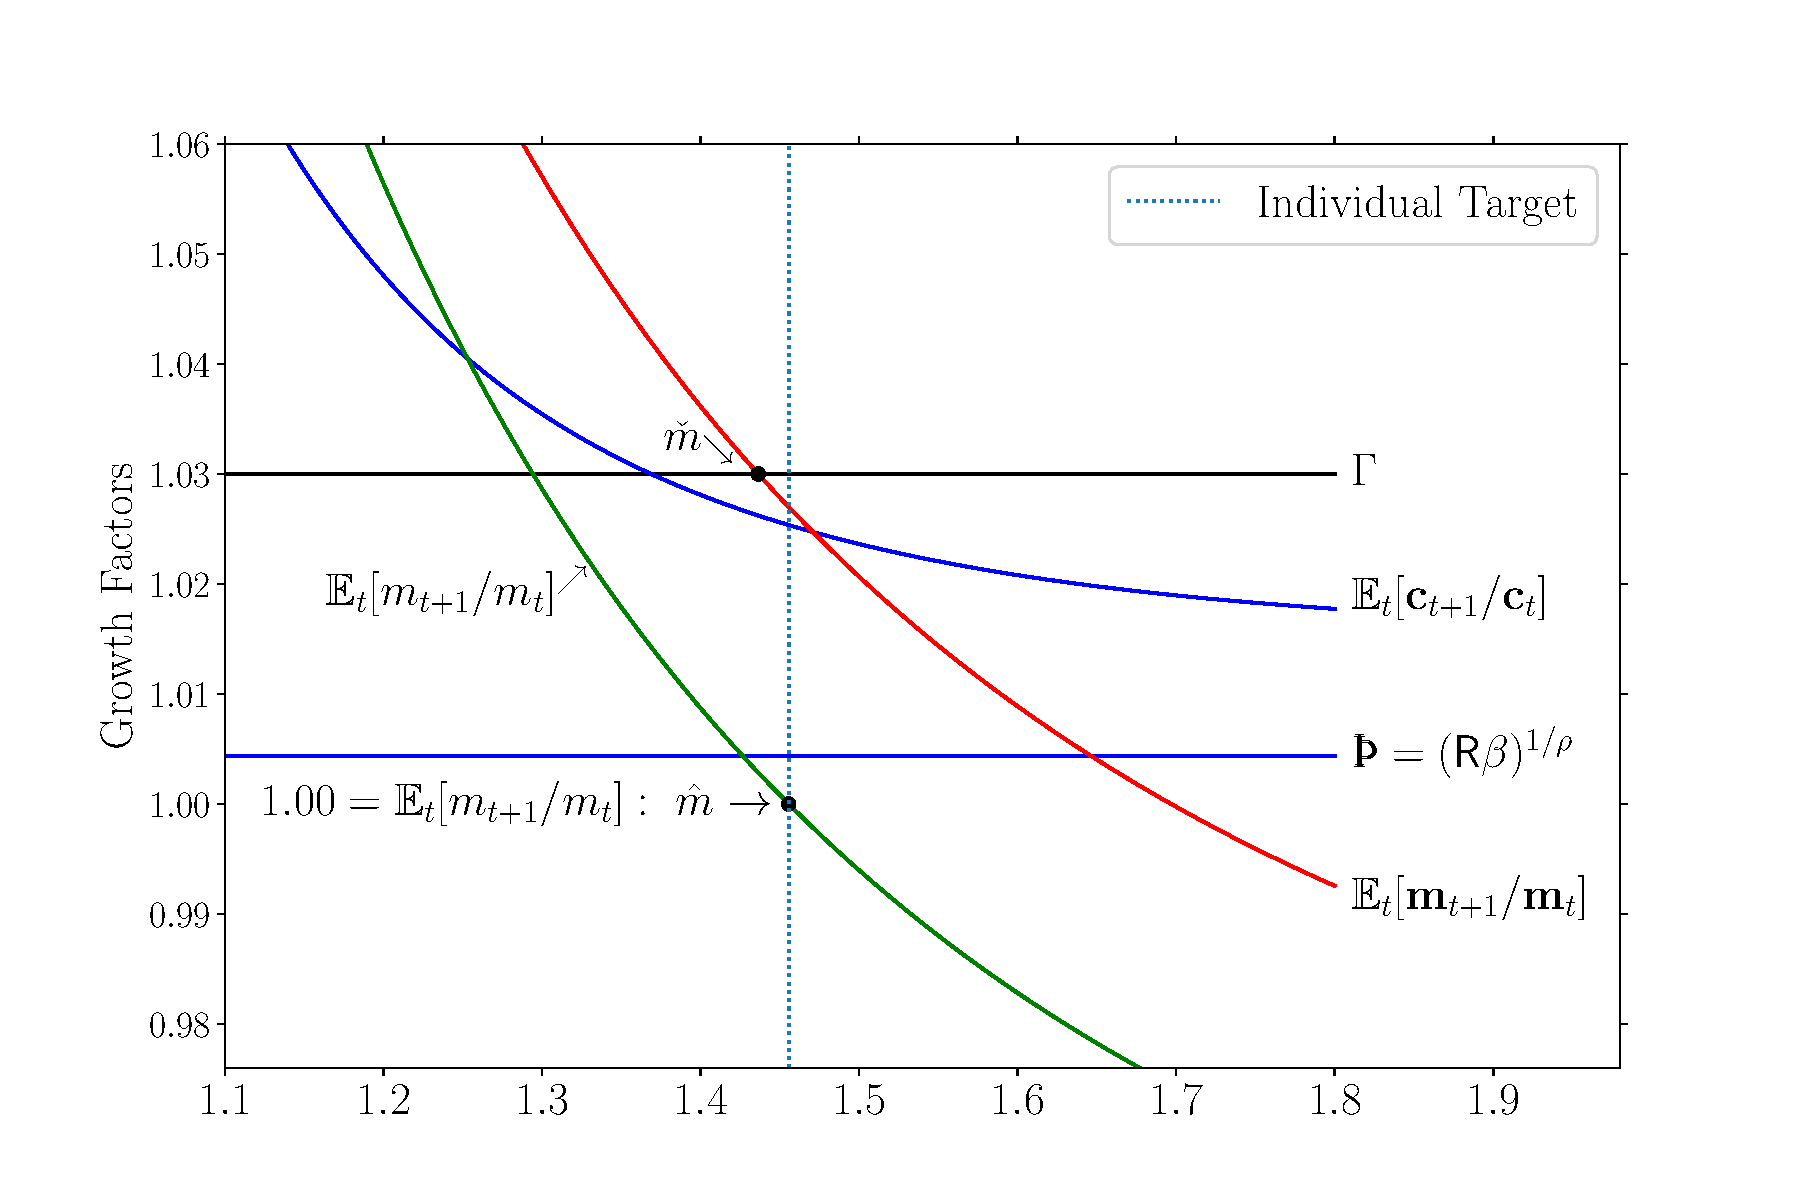
\includegraphics[width=4in]{\FigDir/cNrmTargetFig.pdf}}
\end{frame}

\subsection{Bounds On The Consumption Function}
\begin{frame}
\frametitle{Bounds On the Consumption Function}
\centerline{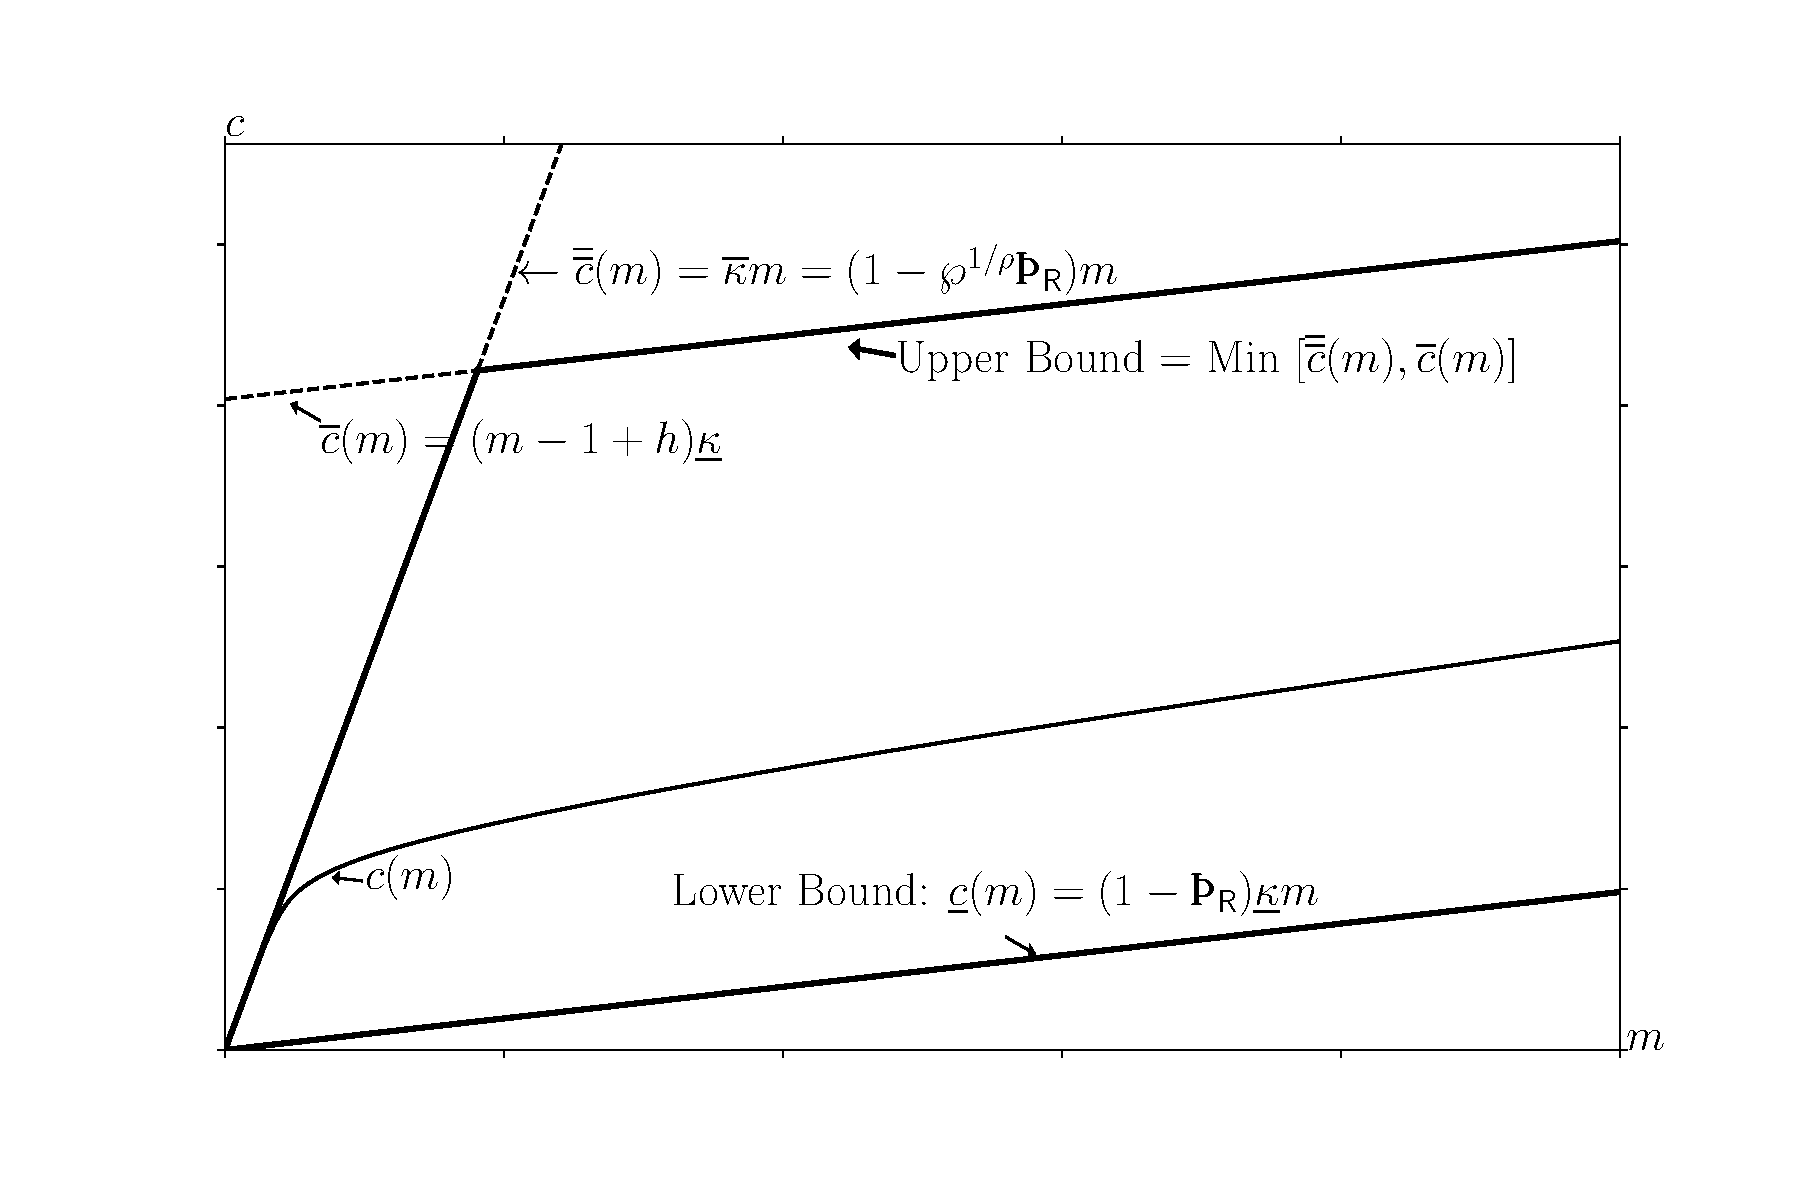
\includegraphics[width=4in]{\FigDir/cFuncBounds.pdf}}
\end{frame}

\begin{frame}
\frametitle{The Marginal Propensity to Consume}
\centerline{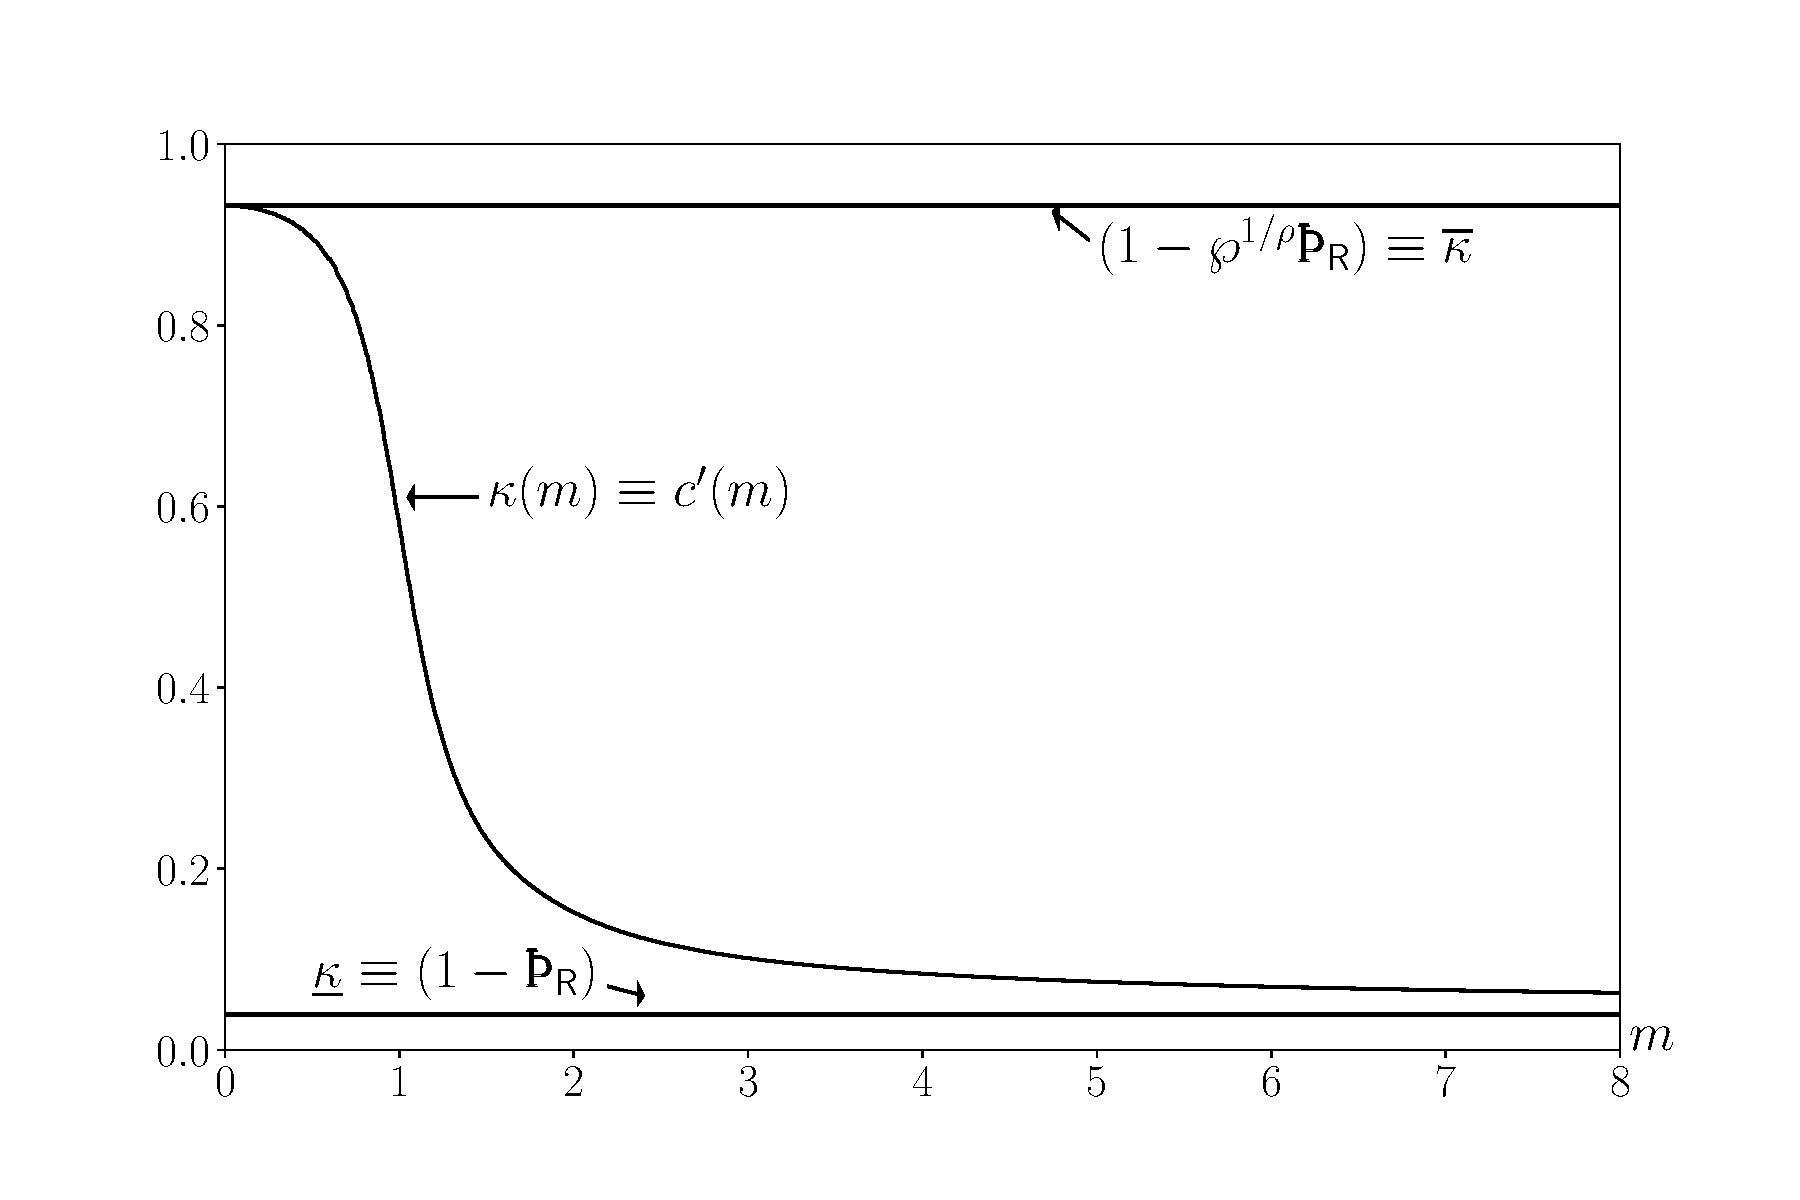
\includegraphics[width=4in]{\FigDir/MPCLimits.pdf}}
\end{frame}

\subsection{The Consumption Function and Target Wealth}
\begin{frame}
\frametitle{The Consumption Function and Target Wealth}
\centerline{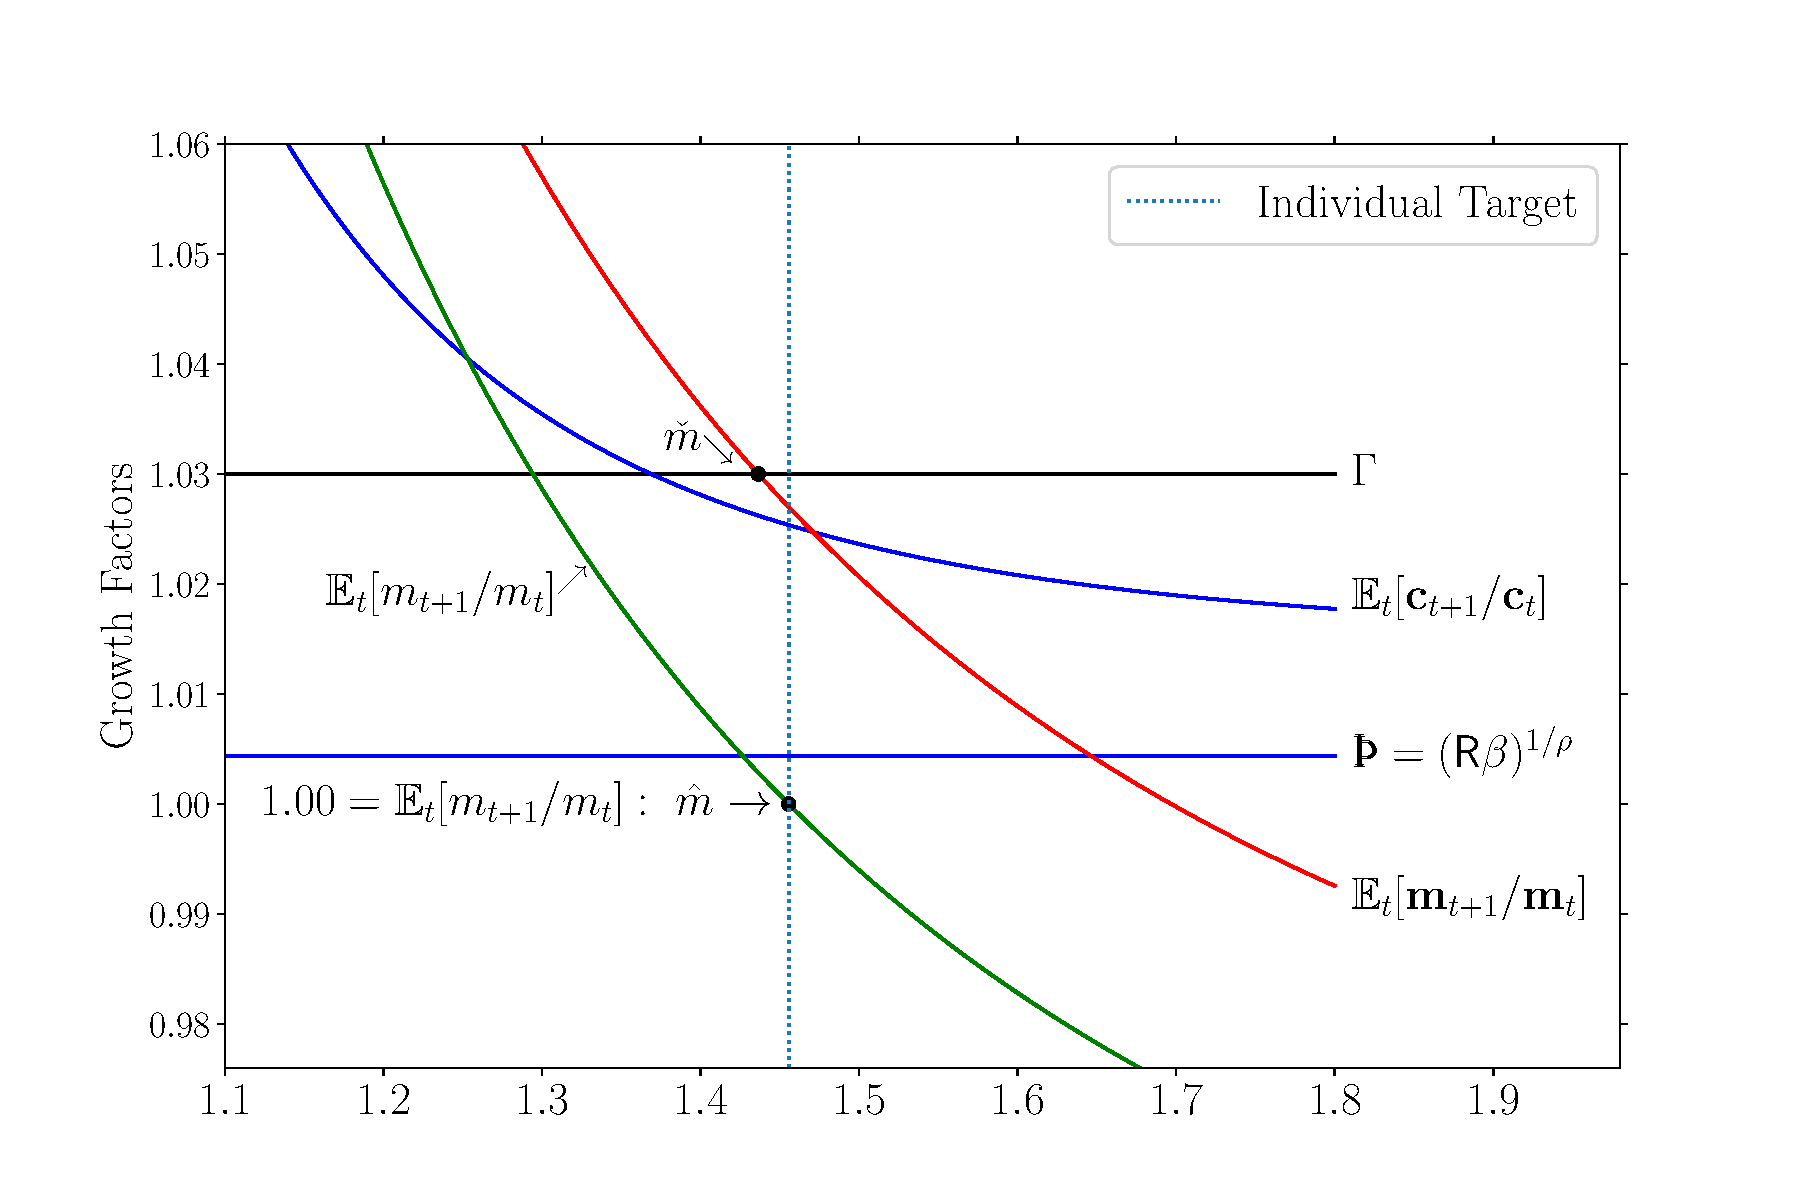
\includegraphics[width=4in]{\FigDir/cNrmTargetFig.pdf}}
\end{frame}



\section{A Small Open Buffer Stock Economy}

\subsection{The Invariant Distribution}
\begin{frame}
\frametitle{Convergence To The Invariant Distribution}

\cite{szeidlInvariant} Proves Existence of an Invariant Distribution of 
$\mNrm, \cNrm, \aNrm,$ etc.

\centerline{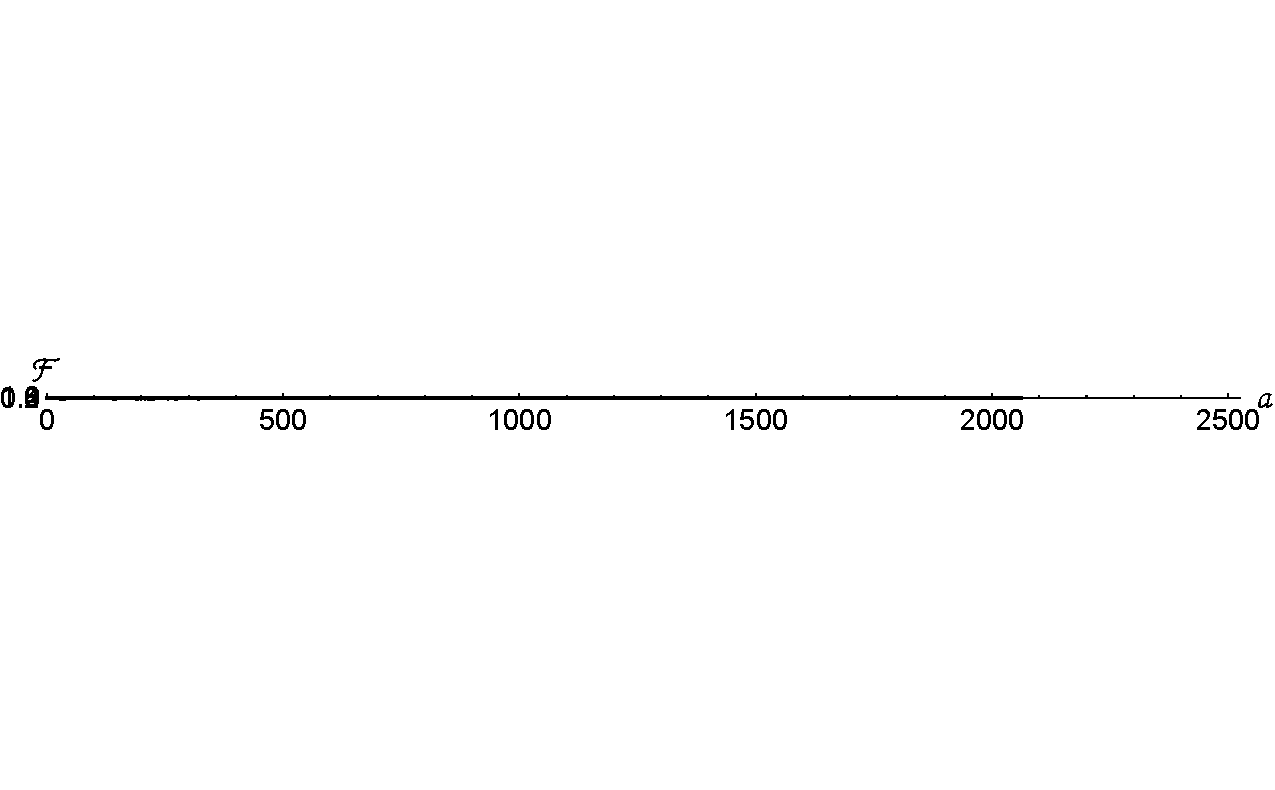
\includegraphics[height=2.5in]{\FigDir/SimCDFsConverge.pdf}}



\end{frame}


\subsection{Balanced Growth Equilbrium}
\begin{frame}
\frametitle{Balanced Growth Equilibrium}

Achieved When Cross Section Distribution Reaches Invariance
\begin{eqnarray}
  \YLvl_{t+1}/\YLvl_{t} = \CLvl_{t+1}/\CLvl_{t} & = & \PermGroFac
\end{eqnarray}

Fisherian Separation Fails, Even Without Liquidity Constraints!
\medskip\medskip

\pause Insight:
\begin{itemize}
\item  Precautionary Saving $\approx$ Liquidity Constraints
\item If $\cnstr{\cFunc}(\mNrm)$ is solution for constrained consumer, 
\end{itemize}
\pause
\begin{equation}
\lim_{ \wp \downarrow 0} \cFunc(\mNrm;\wp) = \cnstr{\cFunc}(\mNrm)
\end{equation}


\end{frame}

\begin{frame}
\frametitle{The MPC Out Of Permanent Shocks}

\url{https://www.econ2.jhu.edu/people/ccarroll/papers/MPCPerm.pdf}
\medskip

Lots of Recent Papers Trying to Measure the MPCP

\medskip
Paper Proves:

\begin{itemize}
\item MPCP $< 1$
\item But not a lot less:
\begin{itemize}
\item 0.75 to 0.95 (annual rate) for wide range of parameter values
\end{itemize}
\end{itemize}

\end{frame}

\section{Conclusions}
\begin{frame}

\begin{itemize}
\item Defined Conditions Under Which Widely Used Problem Has Solution
\begin{itemize}
\item Finite Value of Autarky Condition Guarantees Contraction (with $\WRIC$)
\item Growth Impatience Condition Prevents $m \rightarrow \infty$
\end{itemize}
\item Economy Of Buffer Stock Consumers Exhibits Balanced Growth
\begin{itemize}
\item Even In Absence of General Equilibrium Adj of Interest Rate
\end{itemize}
\end{itemize}

\end{frame}

\def\newblock{\hskip .11em plus .33em minus .07em}

\begin{frame}

\renewcommand{\bibsection}{\subsubsection*{\bibname }}

\tiny 


\pagebreak% Allows two (optional) supplements to hard-wired \texname.bib bibfile:
% economics.bib is a default bibfile that supplies anything missing elsewhere
% Add-Refs.bib is an override bibfile that supplants anything in \texfile.bib or economics.bib
\IfFileExists{\econtexRoot/Add-Refs.bib}{
  % then 
  \typeout{References in Add-Refs.bib will take precedence over those elsewhere}
  \setboolean{AddRefsExists}{true}
  \setboolean{NeitherExists}{false} % Default is true
}{
  % else
  \setboolean{AddRefsExists}{false} % No added refs exist so defaults will be used
  \setboolean{BothExist}{false}     % Default is that Add-Refs and economics.bib both exist
}

% Deal with case where economics.bib is found by kpsewhich 
\IfFileExists{/usr/local/texlive/texmf-local/bibtex/bib/economics.bib}{
  % then
  \typeout{References in default global economics.bib will be used for items not found elsewhere}
  \setboolean{economicsExists}{true}
  \setboolean{NeitherExists}{false}
}{
  % else 
  \typeout{Found no global database file}
  \setboolean{economicsExists}{false}
  \setboolean{BothExist}{false}
}

\IfFileExists{economics.bib}{
  % then
  \typeout{References in economics.bib will be used for items not found elsewhere}
  \setboolean{economicsExists}{true}
  \setboolean{NeitherExists}{false}
}{
  % else 
  \typeout{Found no global database file}
  \setboolean{economicsExists}{false}
  \setboolean{BothExist}{false}
}

\ifthenelse{\boolean{BothExist}}{
  % then use both
  \typeout{bibliography{\econtexRoot/Add-Refs,\econtexRoot/\texname,economics}}
  \bibliography{\econtexRoot/Add-Refs,\econtexRoot/\texname,economics}
  % else both do not exist
}{ % maybe neither does?
  \ifthenelse{\boolean{NeitherExists}}{
    \typeout{bibliography{\texname}}
    \bibliography{\texname}}{
    % no -- at least one exists
    \ifthenelse{\boolean{AddRefsExists}}{
      \typeout{bibliography{\econtexRoot/Add-Refs,\econtexRoot/\texname}}
      \bibliography{\econtexRoot/Add-Refs,\econtexRoot/\texname}}{
      \typeout{bibliography{\econtexRoot/\texname,economics}}
      \bibliography{         \econtexRoot/\texname,economics}}
  } % end of picking the one that exists
} % end of testing whether neither exists


\end{frame}
\end{document}\endinput

% Local Variables:
% TeX-master-file: t
% eval: (setq TeX-command-list  (assq-delete-all (car (assoc "BibTeX" TeX-command-list)) TeX-command-list))
% eval: (setq TeX-command-list  (assq-delete-all (car (assoc "Biber"  TeX-command-list)) TeX-command-list))
% eval: (setq TeX-command-list  (remove '("BibTeX" "%(bibtex) ../LaTeX/%s"    TeX-run-BibTeX nil t :help "Run BibTeX") TeX-command-list))
% eval: (setq TeX-command-list  (remove '("BibTeX"    "bibtex ../LaTeX/%s"    TeX-run-BibTeX nil (plain-tex-mode latex-mode doctex-mode ams-tex-mode texinfo-mode context-mode)  :help "Run BibTeX") TeX-command-list))
% eval: (setq TeX-command-list  (remove '("BibTeX" "bibtex ../LaTeX/%s"    TeX-run-BibTeX nil t :help "Run BibTeX") TeX-command-list))
% eval: (add-to-list 'TeX-command-list '("BibTeX" "bibtex LaTeX/%s" TeX-run-BibTeX nil t                                                                              :help "Run BibTeX") t)
% eval:  (add-to-list 'TeX-command-list '("BibTeX" "bibtex LaTeX/%s" TeX-run-BibTeX nil (plain-tex-mode latex-mode doctex-mode ams-tex-mode texinfo-mode context-mode) :help "Run BibTeX") t)
% TeX-PDF-mode: t
% TeX-file-line-error: t
% TeX-debug-warnings: t
% LaTeX-command-style: (("" "%(PDF)%(latex) %(file-line-error) %(extraopts) -output-directory=./LaTeX %S%(PDFout)"))
% TeX-source-correlate-mode: t
% TeX-parse-self: t
% TeX-parse-all-errors: t
% eval: (cond ((string-equal system-type "darwin") (progn (setq TeX-view-program-list '(("Skim" "/Applications/Skim.app/Contents/SharedSupport/displayline -b %n LaTeX/%o %b"))))))
% eval: (cond ((string-equal system-type "gnu/linux") (progn (setq TeX-view-program-list '(("Evince" "evince --page-index=%(outpage) LaTeX/%o"))))))
% eval: (cond ((string-equal system-type "gnu/linux") (progn (setq TeX-view-program-selection '((output-pdf "Evince"))))))
